\section{Indeling van Windturbines en Bekabeling}
\subsection{Kavelindeling}
Voor de kavelindeling hebben we gekozen voor 48 turbines per kavel, omdat dit het maximale bereik van onze swept area is. Het maximale oppervlak volgens het kavelbesluit is vastgesteld op 2624613 m\textsuperscript{2}, en met 48 turbines beslaan we 2607609,87 m\textsuperscript{2}. Elke turbine bestrijkt een oppervlakte van 54325,20556 m\textsuperscript{2}, berekend met de formule:

\[
\text{{Swept area per turbine}} = \pi \left(\frac{{\text{{Rotor diameter (m)}}}}{2}\right)^2
\]

waarbij de rotor diameter gelijk is aan 263 m volgens de datasheet van NREL 18MW.

De plaatsing van turbines is zo gedaan dat alle obstakels in figuur \ref{fig:windparkitems} worden vermeden. Ook hebben wij een aantal objecten moeten verwijderen (zie figuur \ref{fig:removed-items} om ruimte te maken voor de turbines met bekabeling.
\begin{table}[h]
    \centering
    \begin{tabular}{|c|c|}
        \hline
        \textbf{Point} & \textbf{Function} \\
        \hline
        Q3 P6C & Removed \\
        \hline
        BH01 & Removed \\
        \hline
        BH06 & Removed \\
        \hline
        BH08 & Removed \\
        \hline
        BH09 & Removed \\
        \hline
        BH11 & Removed \\
        \hline
        Q4 & Removed \\
        \hline
        BH12 & Removed \\
        \hline
    \end{tabular}
    \caption{Example of Removed Items}
    \label{tab:removed-items}
\end{table}

Wij hebben de turbines ontworpen met voldoende ruimte tussen de turbines om het lager park effect te minimaliseren. De configuratie van de 48 turbines per kavel is te zien in is in figuur \ref{fig:windparkturbines}.
\begin{figure}[h]
    \centering
    \begin{subfigure}{0.5\textwidth}
        \centering
        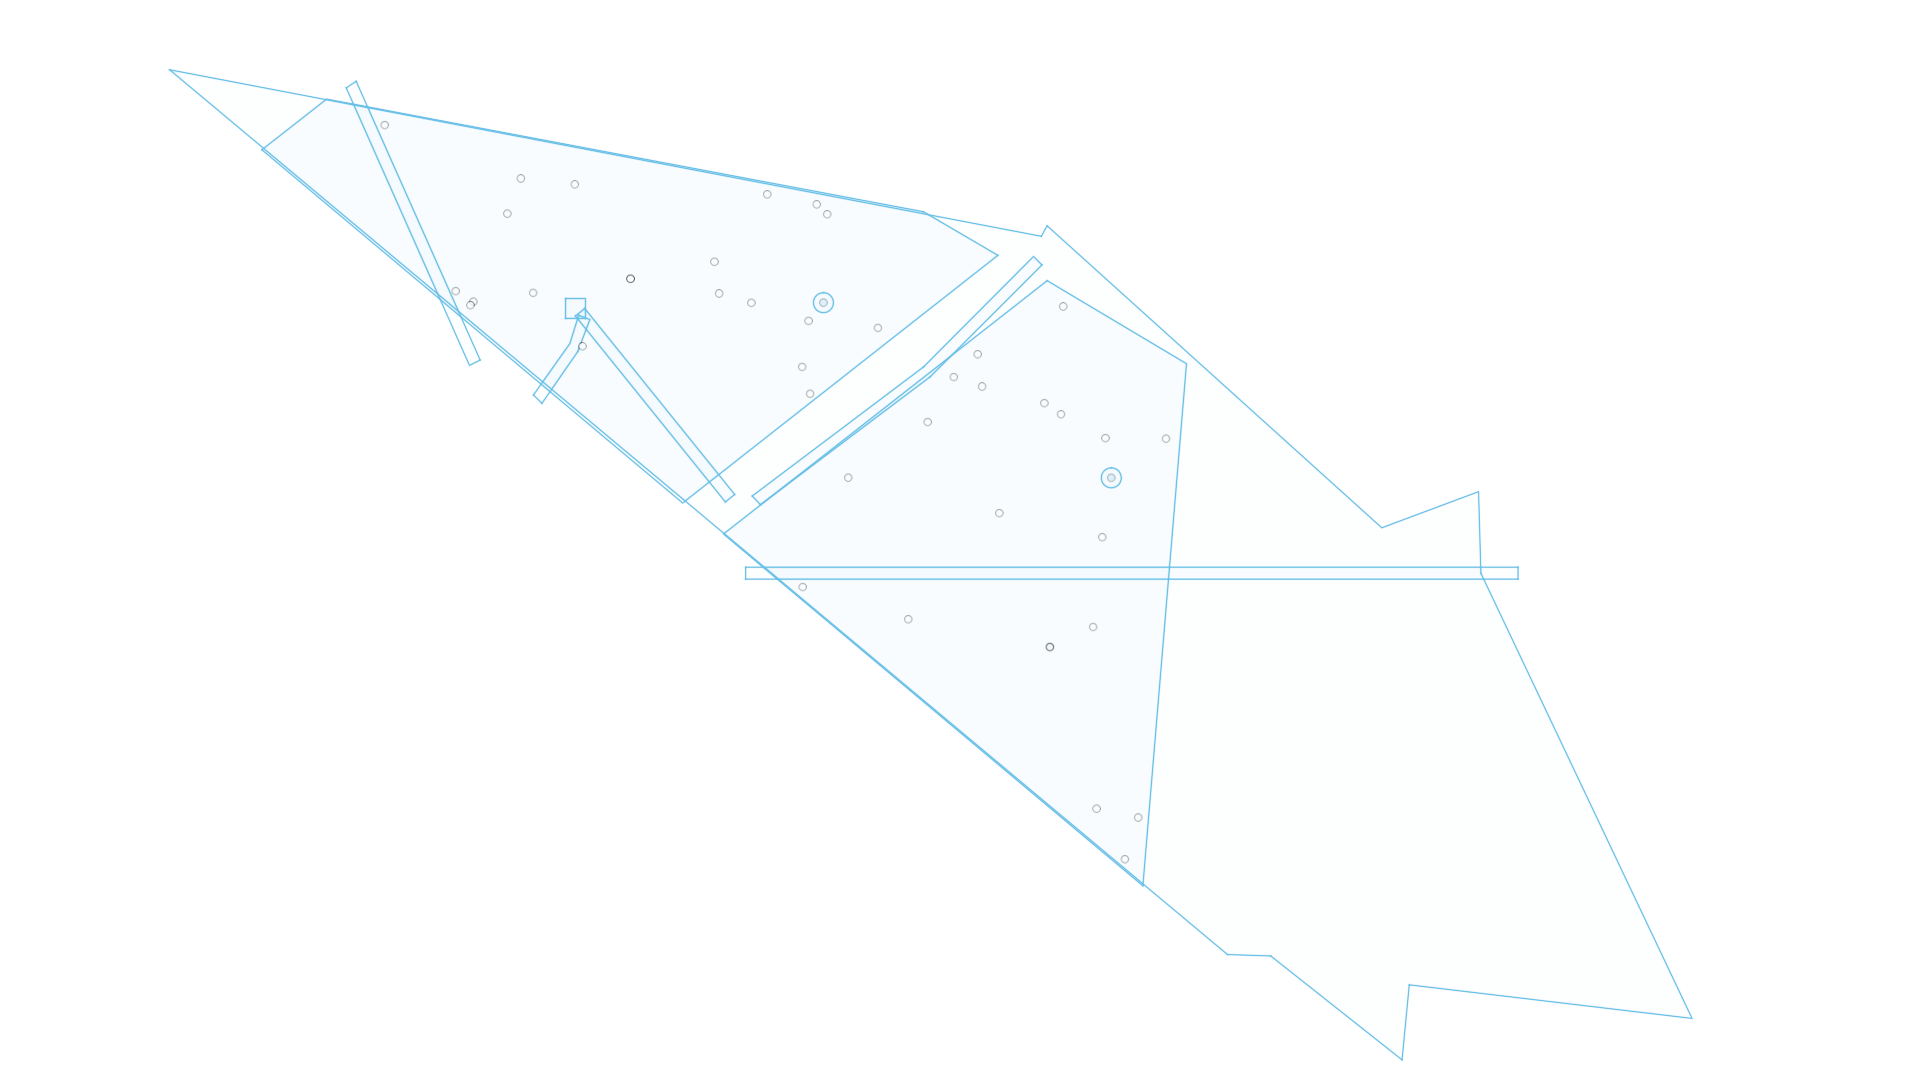
\includegraphics[width=1\textwidth, angle=270]{IMG/Kavelindeling/Windpark v30_BG.png}
        \caption{Alle obstakels aanwezig in kavels.}
        \label{fig:windparkitems}
    \end{subfigure}%
    \begin{subfigure}{0.5\textwidth}
        \centering
        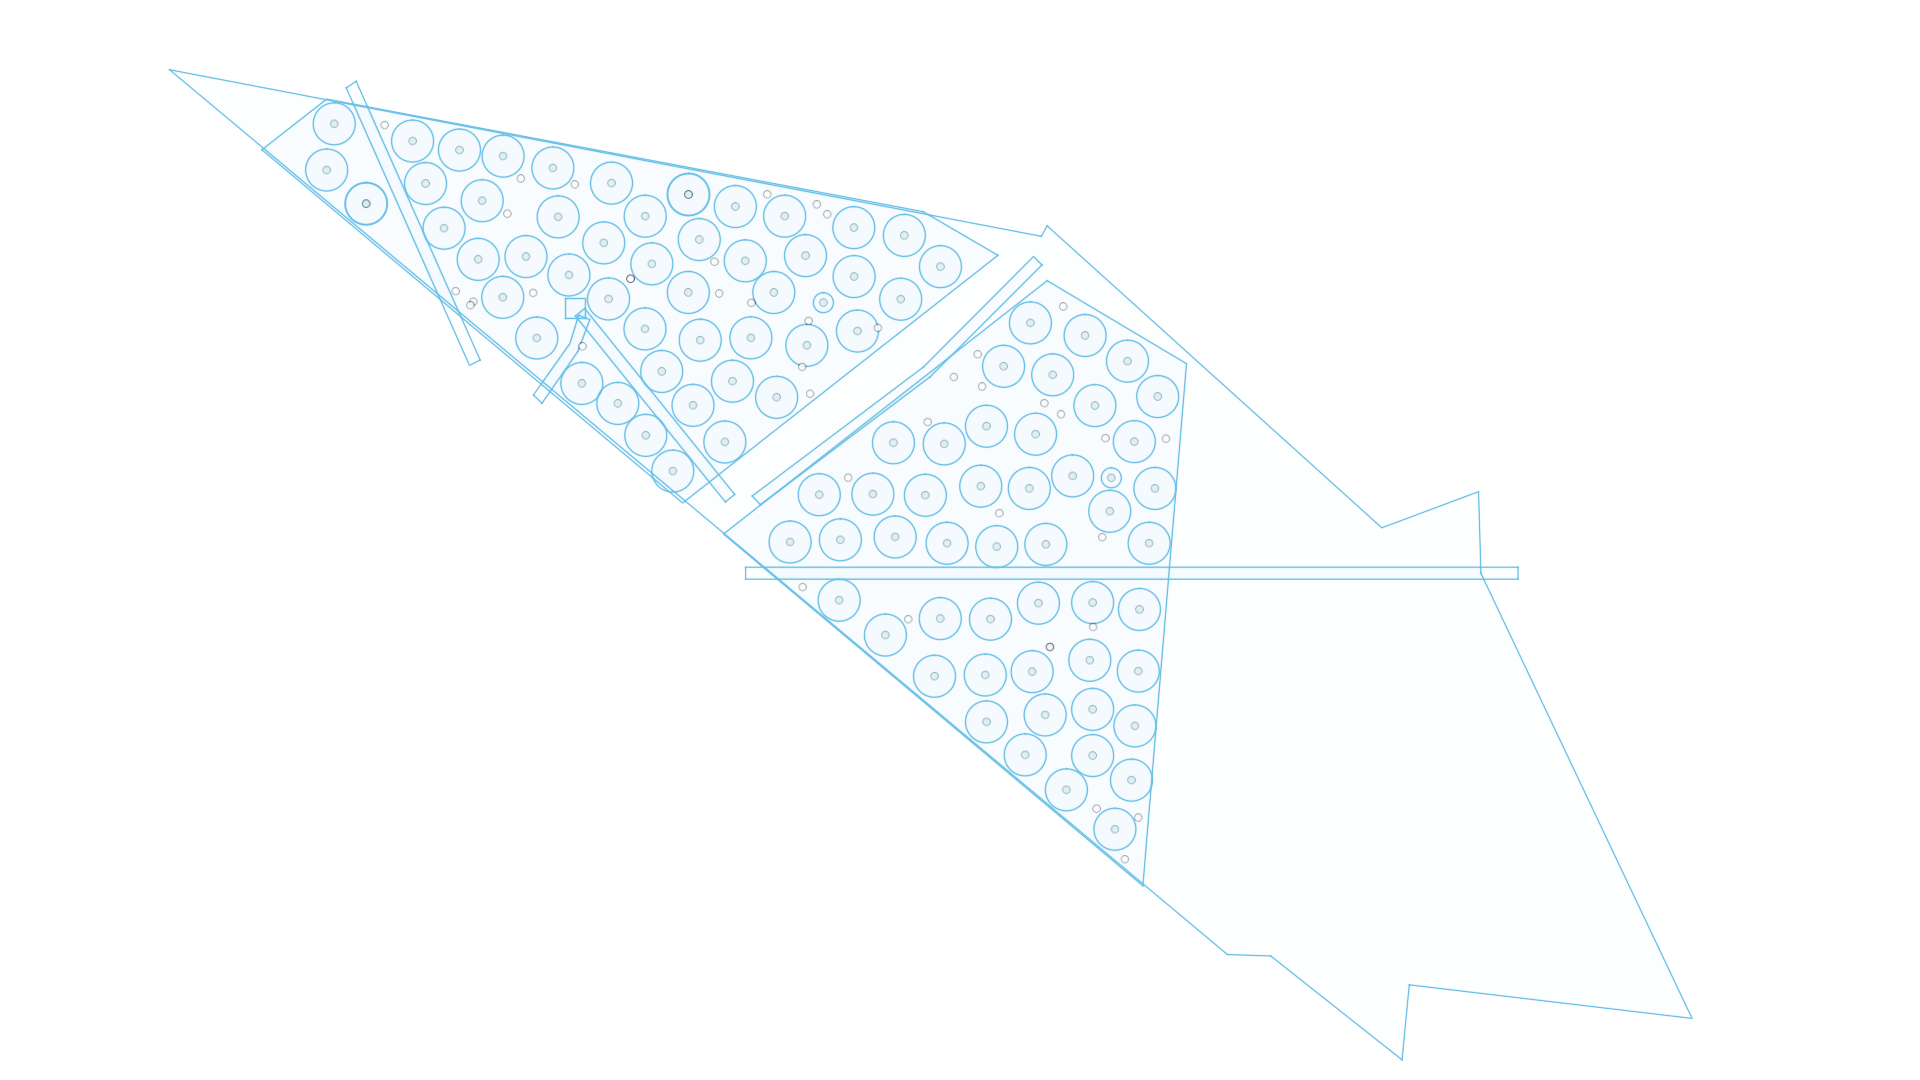
\includegraphics[width=1\textwidth, angle=270]{IMG/Kavelindeling/Windpark v30turbines.png}
        \caption{Alle obstakels en geplaatste turbines.}
        \label{fig:windparkturbines}
    \end{subfigure}
    \caption{Gegevens van het windpark.}
    \label{fig:windpark}
\end{figure}


\subsection{Bekabeling en Vermogen}
De door ons gekozen ABB-kabel is ontworpen voor 66 kV (66000 V). Volgens de datasheet van ABB kunnen we maximaal 825 ampère per kabel overbrengen. Elke turbine levert een vermogen van 18 MW. De formule voor het berekenen van het maximale vermogen per kabel is:

\[
\text{{Maximaal vermogen per kabel}} = \left(\frac{{\text{{Spanning}}}}{{\sqrt{3}}}\right) \times 3 \times \text{{Stroom}} \times \text{{Formfactor}}
\]

Met een veiligheidsfactor (formfactor) van 0,77 wordt dit:

\[
\left(\frac{{66000}}{{\sqrt{3}}}\right) \times 3 \times 825 \times 0,77 = 72618828,18
\]

Dit is het maximale vermogen dat we per kabel/tak kunnen doorsturen. Door de formule \(\frac{{\text{{Turbine MW}}}}{{\text{{Tak MW}}}}\) toe te passen, vinden we dat we veilig 4 turbines per kabel naar het TenneT-station kunnen verbinden.

De bekabeling is weergegeven in figuur \ref{fig:windparktotaal}.

\begin{figure}[H]
\centering
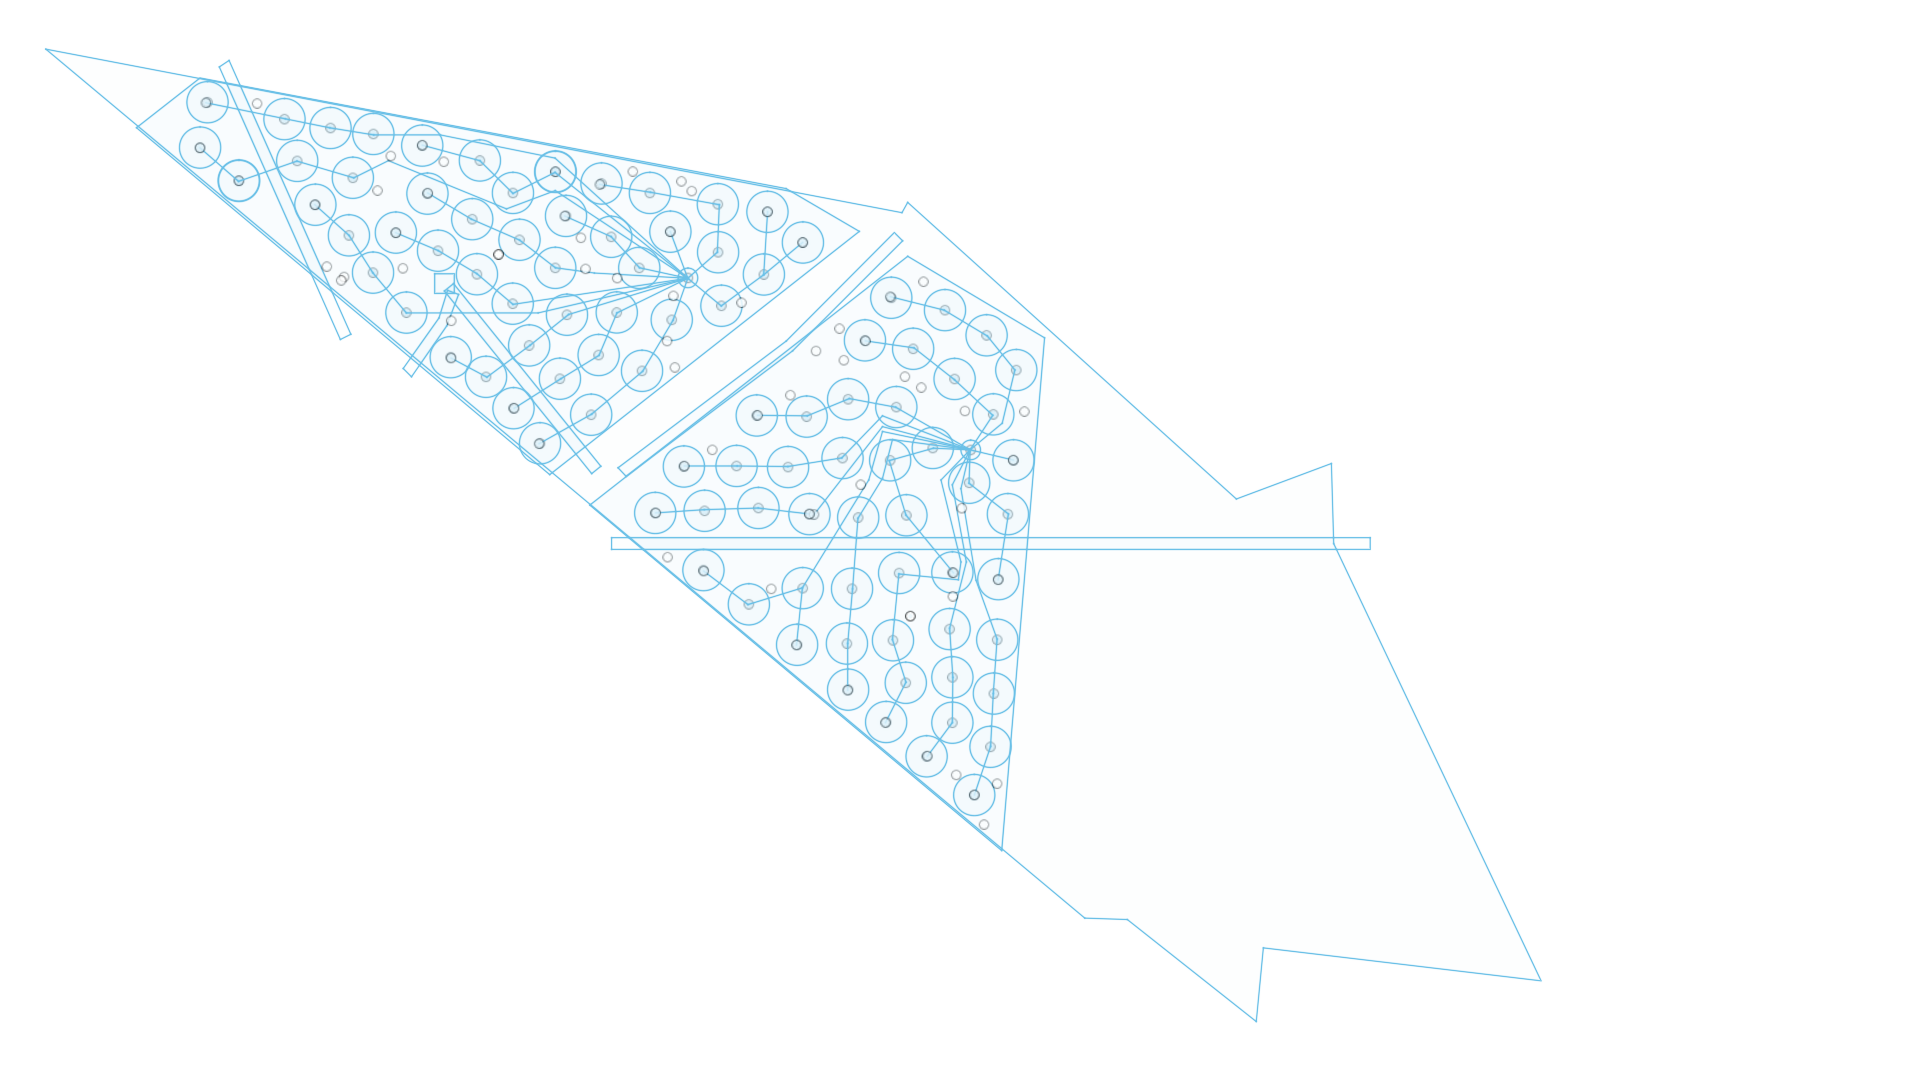
\includegraphics[width=0.5\textwidth, angle=270]{IMG/Kavelindeling/Windpark v30.png}
\caption{Alle obstakels, geplaatste turbines en kabels.}
\label{fig:windparktotaal}
\end{figure}

\subsection{Lengte en Kenmerken van Kabels}
Volgens de heer Dhirhadj Djairam kunnen we elke tak beschouwen als één kabel. Door alle lengtes op te tellen, kunnen we de weerstanden, capaciteiten en inducties van de kabels van kavel VI en VII berekenen. De specifieke weerstand van de kabel wordt bepaald door de formule:

\[
\text{{Specifieke weerstand kabel}} = \frac{{\text{{Lengte kabel}} \times \text{{Specifieke weerstand per km}}}}{{\text{{Doorsnede kabel}}}}
\]

De capaciteit van de kabel wordt gegeven door:

\[
\text{{Capaciteit kabel}} = \text{{Lengte kabel}} \times \text{{Capaciteit per km}}
\]

En de inductie van de kabel is:

\[
\text{{Inductie kabel}} = \text{{Lengte kabel}} \times \text{{Inductie per km}}
\]

Door deze formules toe te passen, kunnen we de gegevens voor kabel VI en VII bepalen, weergegeven in tabel \ref{tab:Kavel VI - Kabel data} en tabel \ref{tab:Kavel VII - Kabel data}.

\begin{table}[h]
\resizebox{\textwidth}{!}{
\begin{tabular}{|llllllllllllll|}
\hline
\rowcolor[HTML]{9B9B9B} 
\multicolumn{14}{|c|}{\cellcolor[HTML]{9B9B9B}\textbf{Kavel VI}} \\ \hline
\rowcolor[HTML]{C0C0C0} 
\multicolumn{1}{|l|}{\cellcolor[HTML]{C0C0C0}\textit{\textbf{Kabel}}} &
  \multicolumn{1}{l|}{\cellcolor[HTML]{C0C0C0}\textit{\textbf{1}}} &
  \multicolumn{1}{l|}{\cellcolor[HTML]{C0C0C0}\textit{\textbf{2}}} &
  \multicolumn{1}{l|}{\cellcolor[HTML]{C0C0C0}\textit{\textbf{3}}} &
  \multicolumn{1}{l|}{\cellcolor[HTML]{C0C0C0}\textit{\textbf{4}}} &
  \multicolumn{1}{l|}{\cellcolor[HTML]{C0C0C0}\textit{\textbf{5}}} &
  \multicolumn{1}{l|}{\cellcolor[HTML]{C0C0C0}\textit{\textbf{6}}} &
  \multicolumn{1}{l|}{\cellcolor[HTML]{C0C0C0}\textit{\textbf{7}}} &
  \multicolumn{1}{l|}{\cellcolor[HTML]{C0C0C0}\textit{\textbf{8}}} &
  \multicolumn{1}{l|}{\cellcolor[HTML]{C0C0C0}\textit{\textbf{9}}} &
  \multicolumn{1}{l|}{\cellcolor[HTML]{C0C0C0}\textit{\textbf{10}}} &
  \multicolumn{1}{l|}{\cellcolor[HTML]{C0C0C0}\textit{\textbf{11}}} &
  \multicolumn{1}{l|}{\cellcolor[HTML]{C0C0C0}\textit{\textbf{12}}} &
  \textit{\textbf{13}} \\ \hline
\rowcolor[HTML]{FFFFFF} 
\multicolumn{1}{|l|}{\cellcolor[HTML]{FFFFFF}\textbf{Afstand} {[}\textit{KM}{]}} &
  \multicolumn{1}{l|}{\cellcolor[HTML]{FFFFFF}5350,00} &
  \multicolumn{1}{l|}{\cellcolor[HTML]{FFFFFF}5296,00} &
  \multicolumn{1}{l|}{\cellcolor[HTML]{FFFFFF}1272,00} &
  \multicolumn{1}{l|}{\cellcolor[HTML]{FFFFFF}13603,00} &
  \multicolumn{1}{l|}{\cellcolor[HTML]{FFFFFF}8234,00} &
  \multicolumn{1}{l|}{\cellcolor[HTML]{FFFFFF}14003,00} &
  \multicolumn{1}{l|}{\cellcolor[HTML]{FFFFFF}3627,00} &
  \multicolumn{1}{l|}{\cellcolor[HTML]{FFFFFF}7177,00} &
  \multicolumn{1}{l|}{\cellcolor[HTML]{FFFFFF}8034,00} &
  \multicolumn{1}{l|}{\cellcolor[HTML]{FFFFFF}10911,00} &
  \multicolumn{1}{l|}{\cellcolor[HTML]{FFFFFF}6835,00} &
  \multicolumn{1}{l|}{\cellcolor[HTML]{FFFFFF}3724,00} &
  5884,00 \\ \hline
\rowcolor[HTML]{EFEFEF} 
\multicolumn{1}{|l|}{\cellcolor[HTML]{EFEFEF}\textbf{Weerstand} {[}\textit{ohm}{]}} &
  \multicolumn{1}{l|}{\cellcolor[HTML]{EFEFEF}93,63} &
  \multicolumn{1}{l|}{\cellcolor[HTML]{EFEFEF}92,68} &
  \multicolumn{1}{l|}{\cellcolor[HTML]{EFEFEF}22,26} &
  \multicolumn{1}{l|}{\cellcolor[HTML]{EFEFEF}238,05} &
  \multicolumn{1}{l|}{\cellcolor[HTML]{EFEFEF}144,10} &
  \multicolumn{1}{l|}{\cellcolor[HTML]{EFEFEF}245,05} &
  \multicolumn{1}{l|}{\cellcolor[HTML]{EFEFEF}63,47} &
  \multicolumn{1}{l|}{\cellcolor[HTML]{EFEFEF}125,60} &
  \multicolumn{1}{l|}{\cellcolor[HTML]{EFEFEF}140,60} &
  \multicolumn{1}{l|}{\cellcolor[HTML]{EFEFEF}190,94} &
  \multicolumn{1}{l|}{\cellcolor[HTML]{EFEFEF}119,61} &
  \multicolumn{1}{l|}{\cellcolor[HTML]{EFEFEF}65,17} &
  102,97 \\ \hline
\rowcolor[HTML]{FFFFFF} 
\multicolumn{1}{|l|}{\cellcolor[HTML]{FFFFFF}\textbf{Capaciteit} {[}\textit{uF}{]}} &
  \multicolumn{1}{l|}{\cellcolor[HTML]{FFFFFF}2033,00} &
  \multicolumn{1}{l|}{\cellcolor[HTML]{FFFFFF}2012,48} &
  \multicolumn{1}{l|}{\cellcolor[HTML]{FFFFFF}483,36} &
  \multicolumn{1}{l|}{\cellcolor[HTML]{FFFFFF}5169,14} &
  \multicolumn{1}{l|}{\cellcolor[HTML]{FFFFFF}3128,92} &
  \multicolumn{1}{l|}{\cellcolor[HTML]{FFFFFF}5321,14} &
  \multicolumn{1}{l|}{\cellcolor[HTML]{FFFFFF}1378,26} &
  \multicolumn{1}{l|}{\cellcolor[HTML]{FFFFFF}2727,26} &
  \multicolumn{1}{l|}{\cellcolor[HTML]{FFFFFF}3052,92} &
  \multicolumn{1}{l|}{\cellcolor[HTML]{FFFFFF}4146,18} &
  \multicolumn{1}{l|}{\cellcolor[HTML]{FFFFFF}2597,30} &
  \multicolumn{1}{l|}{\cellcolor[HTML]{FFFFFF}1415,12} &
  2235,92 \\ \hline
\rowcolor[HTML]{EFEFEF} 
\multicolumn{1}{|l|}{\cellcolor[HTML]{EFEFEF}\textbf{Inductie} {[}\textit{mH}{]}} &
  \multicolumn{1}{l|}{\cellcolor[HTML]{EFEFEF}1658,50} &
  \multicolumn{1}{l|}{\cellcolor[HTML]{EFEFEF}1641,76} &
  \multicolumn{1}{l|}{\cellcolor[HTML]{EFEFEF}394,32} &
  \multicolumn{1}{l|}{\cellcolor[HTML]{EFEFEF}4216,93} &
  \multicolumn{1}{l|}{\cellcolor[HTML]{EFEFEF}2552,54} &
  \multicolumn{1}{l|}{\cellcolor[HTML]{EFEFEF}4340,93} &
  \multicolumn{1}{l|}{\cellcolor[HTML]{EFEFEF}1124,37} &
  \multicolumn{1}{l|}{\cellcolor[HTML]{EFEFEF}2224,87} &
  \multicolumn{1}{l|}{\cellcolor[HTML]{EFEFEF}2490,54} &
  \multicolumn{1}{l|}{\cellcolor[HTML]{EFEFEF}3382,41} &
  \multicolumn{1}{l|}{\cellcolor[HTML]{EFEFEF}2118,85} &
  \multicolumn{1}{l|}{\cellcolor[HTML]{EFEFEF}1154,44} &
  1824,04 \\ \hline
\end{tabular}
}
\caption{Kabeldata van kavel VI}
\label{tab:Kavel VI - Kabel data}
\end{table}

\begin{table}[h]
\resizebox{\textwidth}{!}{
\begin{tabular}{|lllllllllllllll|}
\hline
\rowcolor[HTML]{9B9B9B} 
\multicolumn{15}{|c|}{\cellcolor[HTML]{9B9B9B}\textbf{Kavel VII}} \\ \hline
\rowcolor[HTML]{C0C0C0} 
\multicolumn{1}{|l|}{\cellcolor[HTML]{C0C0C0}\textit{\textbf{Kabel}}} &
  \multicolumn{1}{l|}{\cellcolor[HTML]{C0C0C0}\textit{\textbf{1}}} &
  \multicolumn{1}{l|}{\cellcolor[HTML]{C0C0C0}\textit{\textbf{2}}} &
  \multicolumn{1}{l|}{\cellcolor[HTML]{C0C0C0}\textit{\textbf{3}}} &
  \multicolumn{1}{l|}{\cellcolor[HTML]{C0C0C0}\textit{\textbf{4}}} &
  \multicolumn{1}{l|}{\cellcolor[HTML]{C0C0C0}\textit{\textbf{5}}} &
  \multicolumn{1}{l|}{\cellcolor[HTML]{C0C0C0}\textit{\textbf{6}}} &
  \multicolumn{1}{l|}{\cellcolor[HTML]{C0C0C0}\textit{\textbf{7}}} &
  \multicolumn{1}{l|}{\cellcolor[HTML]{C0C0C0}\textit{\textbf{8}}} &
  \multicolumn{1}{l|}{\cellcolor[HTML]{C0C0C0}\textit{\textbf{9}}} &
  \multicolumn{1}{l|}{\cellcolor[HTML]{C0C0C0}\textit{\textbf{10}}} &
  \multicolumn{1}{l|}{\cellcolor[HTML]{C0C0C0}\textit{\textbf{11}}} &
  \multicolumn{1}{l|}{\cellcolor[HTML]{C0C0C0}\textit{\textbf{12}}} &
  \multicolumn{1}{l|}{\cellcolor[HTML]{C0C0C0}\textit{\textbf{13}}} &
  \cellcolor[HTML]{C0C0C0}\textit{\textbf{14}} \\ \hline
\rowcolor[HTML]{FFFFFF} 
\multicolumn{1}{|l|}{\cellcolor[HTML]{EFEFEF}\textbf{Afstand} {[}\textit{KM}{]}} &
  \multicolumn{1}{l|}{\cellcolor[HTML]{FFFFFF}6270,00} &
  \multicolumn{1}{l|}{\cellcolor[HTML]{FFFFFF}4947,00} &
  \multicolumn{1}{l|}{\cellcolor[HTML]{FFFFFF}5812,00} &
  \multicolumn{1}{l|}{\cellcolor[HTML]{FFFFFF}7919,00} &
  \multicolumn{1}{l|}{\cellcolor[HTML]{FFFFFF}9080,00} &
  \multicolumn{1}{l|}{\cellcolor[HTML]{FFFFFF}14126,00} &
  \multicolumn{1}{l|}{\cellcolor[HTML]{FFFFFF}8609,00} &
  \multicolumn{1}{l|}{\cellcolor[HTML]{FFFFFF}8609,00} &
  \multicolumn{1}{l|}{\cellcolor[HTML]{FFFFFF}5463,00} &
  \multicolumn{1}{l|}{\cellcolor[HTML]{FFFFFF}9179,00} &
  \multicolumn{1}{l|}{\cellcolor[HTML]{FFFFFF}8214,00} &
  \multicolumn{1}{l|}{\cellcolor[HTML]{FFFFFF}9021,00} &
  \multicolumn{1}{l|}{\cellcolor[HTML]{FFFFFF}3823,00} &
  1130,00 \\ \hline
\rowcolor[HTML]{EFEFEF} 
\multicolumn{1}{|l|}{\cellcolor[HTML]{EFEFEF}\textbf{Weerstand} {[}\textit{ohm}{]}} &
  \multicolumn{1}{l|}{\cellcolor[HTML]{EFEFEF}109,73} &
  \multicolumn{1}{l|}{\cellcolor[HTML]{EFEFEF}86,57} &
  \multicolumn{1}{l|}{\cellcolor[HTML]{EFEFEF}101,71} &
  \multicolumn{1}{l|}{\cellcolor[HTML]{EFEFEF}138,58} &
  \multicolumn{1}{l|}{\cellcolor[HTML]{EFEFEF}158,90} &
  \multicolumn{1}{l|}{\cellcolor[HTML]{EFEFEF}247,21} &
  \multicolumn{1}{l|}{\cellcolor[HTML]{EFEFEF}150,66} &
  \multicolumn{1}{l|}{\cellcolor[HTML]{EFEFEF}150,66} &
  \multicolumn{1}{l|}{\cellcolor[HTML]{EFEFEF}95,60} &
  \multicolumn{1}{l|}{\cellcolor[HTML]{EFEFEF}160,63} &
  \multicolumn{1}{l|}{\cellcolor[HTML]{EFEFEF}143,75} &
  \multicolumn{1}{l|}{\cellcolor[HTML]{EFEFEF}157,87} &
  \multicolumn{1}{l|}{\cellcolor[HTML]{EFEFEF}66,90} &
  19,78 \\ \hline
\rowcolor[HTML]{FFFFFF} 
\multicolumn{1}{|l|}{\cellcolor[HTML]{FFFFFF}\textbf{Capaciteit} {[}\textit{uF}{]}} &
  \multicolumn{1}{l|}{\cellcolor[HTML]{FFFFFF}2382,60} &
  \multicolumn{1}{l|}{\cellcolor[HTML]{FFFFFF}1879,86} &
  \multicolumn{1}{l|}{\cellcolor[HTML]{FFFFFF}2208,56} &
  \multicolumn{1}{l|}{\cellcolor[HTML]{FFFFFF}3009,22} &
  \multicolumn{1}{l|}{\cellcolor[HTML]{FFFFFF}3450,40} &
  \multicolumn{1}{l|}{\cellcolor[HTML]{FFFFFF}5367,88} &
  \multicolumn{1}{l|}{\cellcolor[HTML]{FFFFFF}3271,42} &
  \multicolumn{1}{l|}{\cellcolor[HTML]{FFFFFF}3271,42} &
  \multicolumn{1}{l|}{\cellcolor[HTML]{FFFFFF}2075,94} &
  \multicolumn{1}{l|}{\cellcolor[HTML]{FFFFFF}3488,02} &
  \multicolumn{1}{l|}{\cellcolor[HTML]{FFFFFF}3121,32} &
  \multicolumn{1}{l|}{\cellcolor[HTML]{FFFFFF}3427,98} &
  \multicolumn{1}{l|}{\cellcolor[HTML]{FFFFFF}1452,74} &
  429,40 \\ \hline
\rowcolor[HTML]{EDEDED} 
\multicolumn{1}{|l|}{\cellcolor[HTML]{EFEFEF}\textbf{Inductie} {[}\textit{mH}{]}} &
  \multicolumn{1}{l|}{\cellcolor[HTML]{EDEDED}1943,70} &
  \multicolumn{1}{l|}{\cellcolor[HTML]{EDEDED}1533,57} &
  \multicolumn{1}{l|}{\cellcolor[HTML]{EDEDED}1801,72} &
  \multicolumn{1}{l|}{\cellcolor[HTML]{EDEDED}2454,89} &
  \multicolumn{1}{l|}{\cellcolor[HTML]{EDEDED}2814,80} &
  \multicolumn{1}{l|}{\cellcolor[HTML]{EDEDED}4379,06} &
  \multicolumn{1}{l|}{\cellcolor[HTML]{EDEDED}2668,79} &
  \multicolumn{1}{l|}{\cellcolor[HTML]{EDEDED}2668,79} &
  \multicolumn{1}{l|}{\cellcolor[HTML]{EDEDED}1693,53} &
  \multicolumn{1}{l|}{\cellcolor[HTML]{EDEDED}2845,49} &
  \multicolumn{1}{l|}{\cellcolor[HTML]{EDEDED}2546,34} &
  \multicolumn{1}{l|}{\cellcolor[HTML]{EDEDED}2796,51} &
  \multicolumn{1}{l|}{\cellcolor[HTML]{EDEDED}1185,13} &
  \cellcolor[HTML]{EFEFEF}350,30 \\ \hline
\end{tabular}
}
\caption{Kabeldata van kavel VII}
\label{tab:Kavel VII - Kabel data}
\end{table}
